\chapter{Methodology}
\label{chap:methodology}

\section{Measurement Process}

The exposed time series of this work represent network end-to-end measures of a
cable-television infrastructure, which runs DOCSIS with asymmetric download and
upload bandwidths. Home routers connected to the cable modem communicate with
one or more servers strategically located by the ISP\@. Measurements results
from
each home router are consolidated every half hour and, by the end of every day,
are transferred to a database. The software responsible for these procedures was
developed by TGR (a startup at COPPE/UFRJ) in collaboration with the university
(UFRJ), and is spread over a customers subset of a major Brazilian ISP\@.

In~\cite{a_preliminary_performance_measurement_study_of_residential_broadband_services_in_brazil},
a preliminary investigation of several metrics is presented. To measure the
round
trip packet loss fraction and RTT between the home router and the associated
server, the
home router sends a train of short UDP packets, and then the server bounces back
them. The data here presented considers a train of 100 UDP packets of 32 bytes,
separated by 1 millisecond. This dissertation only deals with these two
metrics.

The resulted time series are unevenly spaced due to a range of reasons. First,
measurements are initiated only if the residential link is not under use by the
ISP customer. Also, the client may have no Internet connection to start a
measurement, or even be without electrical energy.

TALK ABOUT TOPOLOGY

\section{Supervised Learning Try}

As stated in Chapter~\ref{chap:change_point_detection}, one of the main issues
of this work is the algorithms and parameters selection.
In general, this process requires a dataset to enable the evaluation of an
algorithm setup.

There are several approaches to construct a
change points dataset in the literature.
Some works create simulated time series, in which distinct segments are sampled
by the same generative model with different
parameters~\cite{change_point_detection_in_time_series_data_by_relative_density_ratio_estimation}.
In general, this type of data is more easily handled by change point detection
algorithms, since some methods assume the same models used in the dataset
building process. Also, real data can have complex characteristics that are
difficult to be reproduced by generative models. Another strategy is to join
segments from different real time series with different
characteristics~\cite{inertial_hidden_markov_models_modeling_change_in_multivariate_time_series}.
However, this can introduce unreal change points scenarios.

When the latent information of the time series are available, and if there is a
complete knowledge of what configurations changes in the latent state impact
data, it is possible to check the change points only analyzing this underlying
information. As an example, consider a time series that represents the cardiac
frequency of a soccer player during a match. Also, consider that in this
controlled environment, the only causes of changes in the cardiac frequency are
the variations of physical activities, such as starting or stopping to run.
Therefore,
it is possible to use the times in which a player changed his movement behavior
as the change points, whithout even analyzing the time series. However, in the
application domain of the present work, this approach would be impractical.
First, this would need the expertise of how the configurations of network
topology, routers congestion, physical equipment problems, among other features,
affect the different end-to-end QoS metrics.
Second, this kind of information is absent in the dataset, and would be too
complex to collect it.

The approach followed in this work was to use visual classifications,
as it was done
in~\cite{learning_sparse_penalties_for_change_point_detection_using_max_margin_interval_regression}.
An application domain expert was exposed to a set of time series, and visually
indicated his opinion about the change points locations. It is known that visual
inspection methods can bring erroneous
conclusions~\cite{leveraging_cloud_data_to_mitigate_user_experience_from_breaking_bad},
and also amplify subjectivity, however, it was the best alternative considering
the data availability and the objective of working with real data.

Through a web system the user freely marked the change points with a mouse.
The fact that data is not regularly sampled in time could bring an unwanted
visual change perception. Therefore, the X axis of the displayed time series
represented only the temporal order of the measures.

A single specialist classified all time series.
This person has experience with network measurements and statistical modeling,
however, without background in change point detection.
The user could take any time to make a classification, and it was able to access
the system in different days. Additionally, it was provided a set of tips to the
specialist:

\begin{itemize}
    \item In the case of packet loss fraction, mean changes between 0 and 0.1
    are more sensible to the end users.
    \item The time axis only represents the temporal order of the measurements.
    However, in general, consecutive points in time axis are separated by 30
    minutes.
    \item Outlier is not a statistical change. An outlier is an observation that
    lies outside the overall pattern of a distribution.
\end{itemize}

To provide a clear visualization, the change points dataset was composed by time
series with 10 days of data. Therefore, each time series of the previous dataset
was split in two, one from 01/may/2016 to 10/may/2016, and other from
11/may/2016 to 20/may/2016. Also, it was selected only the ones that have at
least 85\% of the maximum possible number of points during the specified period,
considering that data is sampled at most two times in a hour. Change points can
be interpreted as rare events in this dataset, and most data streams have almost
all measures with zero losses. Therefore, to increase the dataset entropy,
it was only selected time series that have at least one window of length 48 with
more than 5 measures with loss fraction larger than 0.01. These filters resulted
in 522 time series.

Figure~\ref{fig:survey_system} presents a system snapshot.
The vertical red line means that the user marked a change point in that
position.

It is important to note that the algorithms presented in
Chapter~\ref{chap:change_point_detection} doesn't use a previous point labels
for a training phase. Once a change point dataset is constructed, in which a
train set each labels each point of a time series as a change point or not, can
open new possibilities to a supervised learning procedure, in which are not
much explored in the literature of change pointe detection.

\begin{figure}[H]
    \centering
    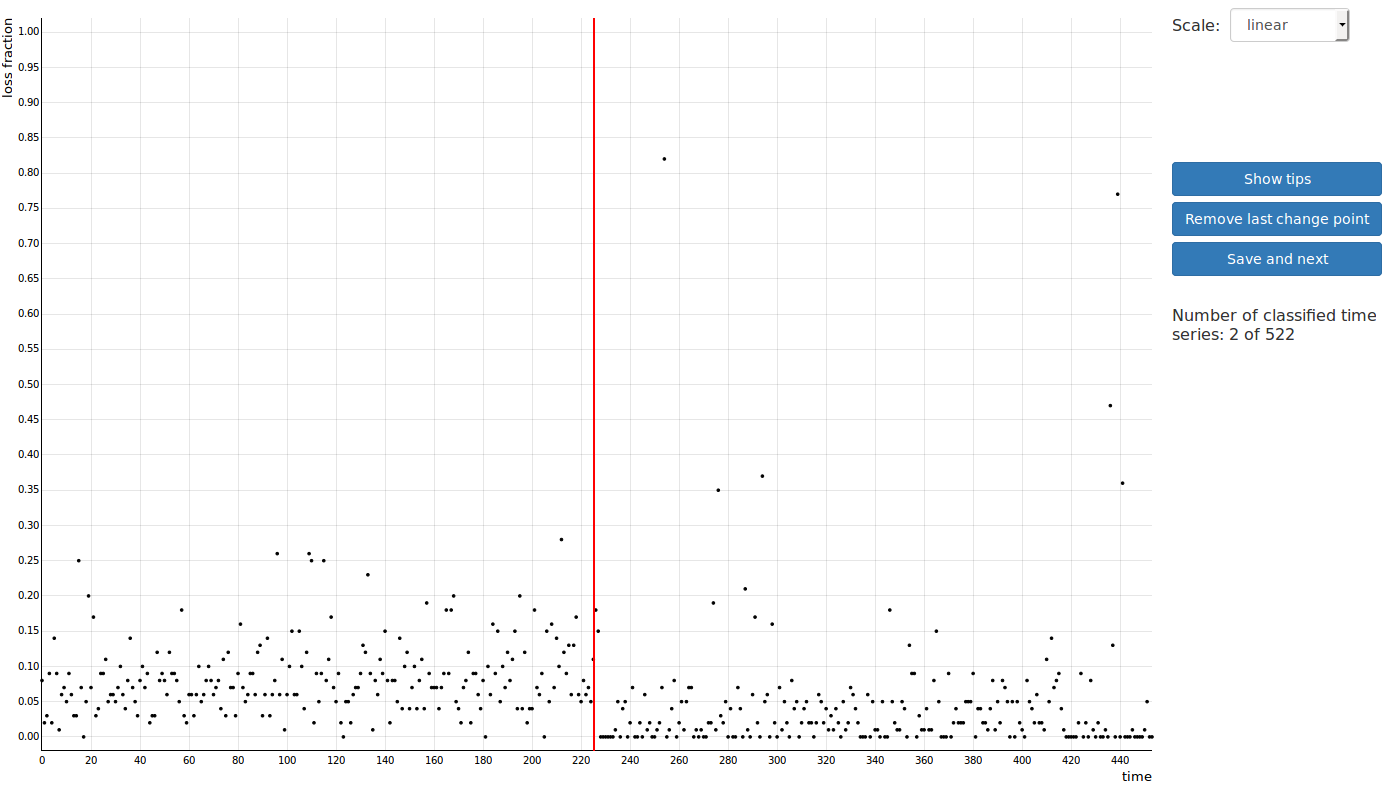
\includegraphics[width=0.9\linewidth]{./figures/methodology/supervised_learning_try/survey_system.png}
    \caption{Survey system snapshot.}
\label{fig:survey_system}
\end{figure}%

\section{Pipeline}

\begin{figure}[H]
    \centering
    \includegraphics[width=0.9\linewidth]{./figures/methodology/pipeline/pipeline.png}
    \caption{Pipeline.}
\label{fig:survey_system}
\end{figure}%

\section{Spatial Aggregation}
\section{Change Point Detection Parameters Tuning}
\section{Time Aggregation}
\section{Spatial/Time Correlation}
\section{Differences to Previous Systems}
